\begin{figure*}[t]
    \centering
    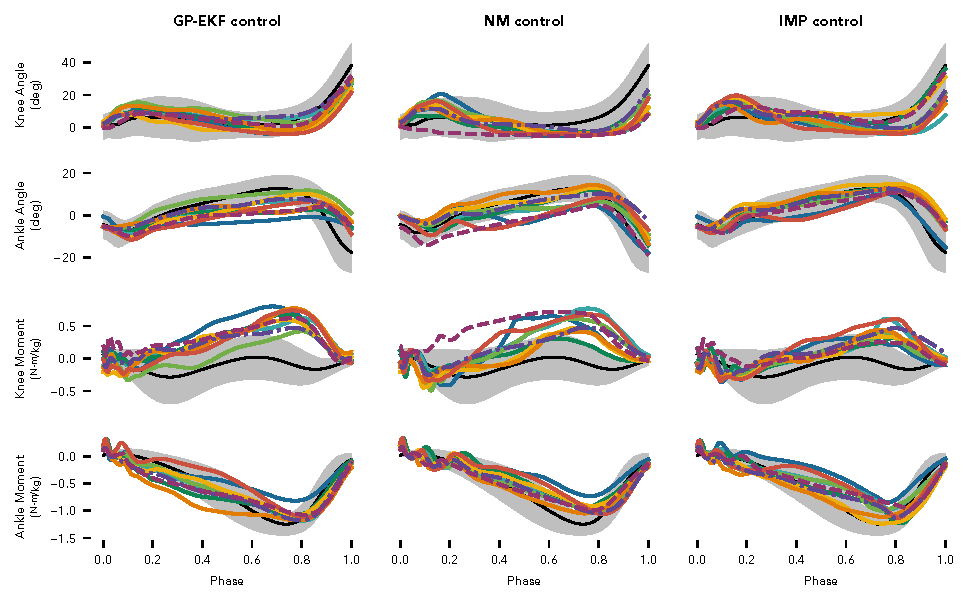
\includegraphics[width=\textwidth]{normal_data} 
    \caption[Ability to reproduce normal walking characteristics]{Ability to
    reproduce normal walking characteristics. Average knee angle (row 1), ankle
    angle (row 2), knee moment (row 3), and ankle moment (row 4) for the GP-EKF
    controller (column 1), neuromuscular controller (column 2), and impedance
    controller (column 3). Black traces and gray shaded areas show the mean and
    two standard deviations for very slow human walking data
    (from~\citep{bovi2011multiple}). Colored lines show individual subject data.
    Amputee gait data indicated by dashed lines and experienced user data
    indicated by dash-dot lines.}\label{fig:controller_comparison}
\end{figure*}

\section{Results}\label{sec:phase_est_results}
\subsection{Ability to Reproduce Normal Walking}

\Cref{fig:controller_comparison} shows the average knee and ankle angles as well
as the corresponding joint moments generated by the prosthesis controllers
during undisturbed walking at \unitfrac[0.8]{m}{s}. All three control strategies
produce knee angle trajectories that are similar to the able-bodied data (first
row). The neuromuscular (NM) control, however, seems to suffer more from knee
over extension during mid-stance and less knee flexion at the end of stance. For
some able-bodied subjects, and to a substantial degree for the amputee subject,
the knee over-extension causes the joint to engage the mechanical hard-stop on
the prosthesis. This triggers a sudden rise in knee torque.
\Cref{fig:kinematic_errors}a summarizes the root-mean-squared (RMS) error
between the mean able-bodied knee kinematics and the median knee kinematics of
each subject. The GP-EKF control strategy produces significantly more
kinematically natural knee angle trajectories, whereas the NM control produces
the least kinematically natural knee trajectories. 

\begin{figure}[t]
   \centering 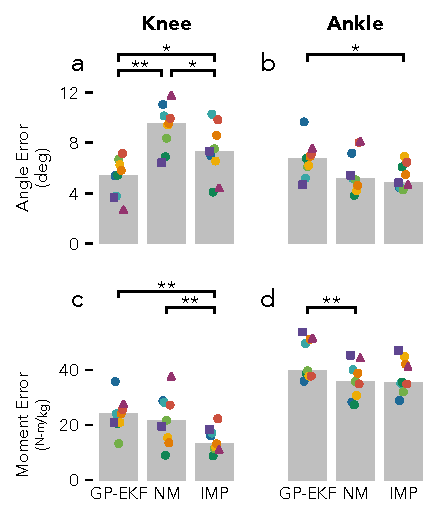
\includegraphics[width=\columnwidth]{kinematic_errors}
   \caption[Average kinematic and kinetic errors]{Average kinematic (a,b) and
   kinetic (c,d) errors produced by the three different controllers compared to
   able-bodied data. GP-EKF produces significantly more natural knee angles than
   NM or IMP control, but slightly less natural ankle angles and joint torques.
   Grey bars show median of subject data, circle markers indicate able-bodied
   subject data, triangle markers indicate amputee data, and square markers
   indicate experienced able-bodied user data. $*: p < 0.05$, $**: p <
   0.01$.}\label{fig:kinematic_errors}
\end{figure}
The second row of~\cref{fig:controller_comparison} shows the average ankle
trajectories for each control strategy. In this case, the GP-EKF control
produced the least accurate trajectories. As shown
in~\cref{fig:kinematic_errors}b, this trend reached statistical significance
compared to impedance (IMP) control, which produced the most natural ankle angle
trajectories. The unnaturalness of the GP-EKF control ankle trajectories is
largely due to (1) a lack of plantar flexion in the push-off phase and (2) a
lack of dorsiflexion during mid-stance for 3 out of 8 subjects, who all chose
the same control surface set.

Finally, the third and fourth row of~\cref{fig:controller_comparison} show the
knee and ankle moments for the three controllers. IMP control produced the most
natural knee moments by a significant margin (\cref{fig:kinematic_errors}c),
whereas the GP-EKF and NM controllers performed comparably. Although the GP-EKF
control produced the least natural ankle moments, the absolute differences were
small (\cref{fig:kinematic_errors}d).

\subsection{Robustness to Ground Height Disturbances}
\begin{marginfigure}
    \centering
    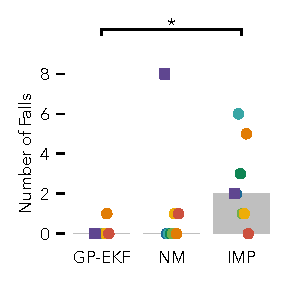
\includegraphics[width=\columnwidth]{num_falls} 
    \caption[Robustness to ground height disturbances]{Robustness to ground
    height disturbances. Number of falls accrued for each controller during
    ground height disturbance trials. GP-EKF control significantly reduced the
    number of falls compared to IMP control.}\label{fig:num_block_falls}
\end{marginfigure}

\Cref{fig:num_block_falls} shows the number of times able-bodied subjects fell
with each control strategy when stepping on blocks. Subjects fell significantly
more often with the IMP control compared to either the GP-EKF or NM controllers.
However, when using the neuromuscular control the experienced user fell 8 times,
more than any other subject in any condition.

\subsection{Adaptability of Phase Estimate}

\begin{marginfigure}
    \centering
    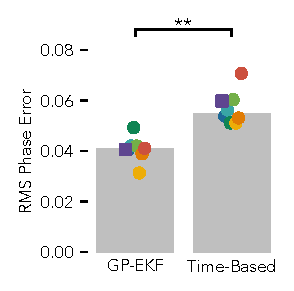
\includegraphics[width=\columnwidth]{phase_error} 
    \caption[Adaptability of phase estimate]{Adaptability of phase estimate.
    Mean phase error of EKF versus time-based phase estimation when walking with
    sinusoidally varying treadmill speed. The EKF significantly improves phase
    tracking compared to the time-based
    estimate.}\label{fig:speed_phase_err_mean}
\end{marginfigure}
The adaptability of the phase estimate was tested by sinusoidally varying the
treadmill speed during walking. \Cref{fig:speed_phase_err_mean} shows the
average RMS errors of the EKF-based phase estimate and time-based phase estimate
compared to the ground-truth phase obtained in hindsight. For all subjects, the
EKF tracked the true phase significantly more accurately than did the time-based
phase estimate.

For a more specific example, \cref{fig:speed_phase_est_sub_1} shows the phase
estimates during the treadmill speed variation experiment for a single subject.
Because the initial conditions of the EKF and the time-based phase estimates are
identical (compare \cref{eq:init_cond_ekf} and \cref{eq:init_cond_time}), the
phase estimates are similar in early stance. As the treadmill speed changes from
one step to the next, the time-based phase estimate diverges significantly from
the true phase. The EKF, on the other hand, is able to recover to the true phase
towards the end of stance and more accurately predicts the toeoff event.
\begin{figure}[t]
    \centering
    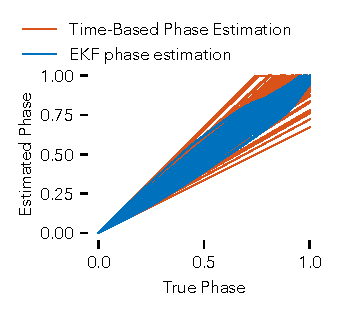
\includegraphics[width=\columnwidth]{speed_phase_err_sub_1} 
    \caption[Example of EKF-based phase estimation versus time-based phase
    estimation for one subject]{Example of EKF-based phase estimation (red)
    versus time-based phase estimation (blue) for one subject. Due to
    step-to-step speed variations caused by the sinusoidally varying treadmill
    speed, the time based phase estimation accrues significant errors.  In
    contrast, the EKF-based phase estimate is able to respond to changes in gait
    within the gait cycle, thus reducing phase estimation
    errors.}\label{fig:speed_phase_est_sub_1}
\end{figure}

\subsection{Response to Sudden Treadmill Stops}
\begin{figure}[t]
    \centering
    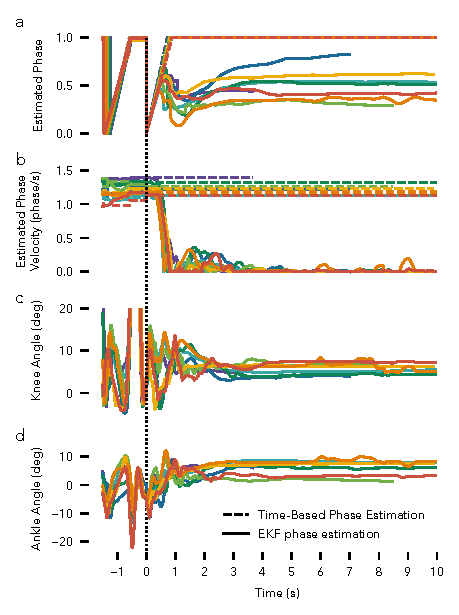
\includegraphics[width=\columnwidth]{stop_plot} 
    \caption[Response to sudden treadmill stops]{Response to sudden treadmill
    stops. Estimated phase (a) and phase velocity (b), and the measured knee (c)
    and ankle (d) angles when the treadmill is suddenly stopped half way through
    stance.  When gait stops, the EKF-estimated phase stabilizes to a constant
    value (solid traces), phase velocity falls to zero, and the joint angles
    approach \unit[5]{deg} as desired by the control surfaces
    (compare~\cref{fig:control_surf}). The time-based phase estimate fails to
    respond (dashed lines). Vertical black dotted line indicates heel strike of
    final stance phase.}\label{fig:stop_plot}
\end{figure}

Finally,~\cref{fig:stop_plot} shows the phase (a), and phase velocity (b)
estimates when the treadmill is suddenly stopped halfway through the stance
phase. The EKF phase estimates (solid lines) reflect the fact that the gait
cycle has halted, as they do not continue to progress to one. Moreover, when
the treadmill stops, the knee (c) and ankle angles (d) approach \unit[5]{deg} as
desired for standing (compare \cref{fig:control_surf}). In contrast, the
time-based phase estimates (dashed lines in panels (a) and (b)) continue at
their initial rate, with the phase reaching one. 
